\documentclass[linenumbers]{aastex631}
\usepackage[utf8]{inputenc}
\usepackage[T1]{fontenc}
\usepackage{graphicx}
\graphicspath{ {./figs_scratch/} }
\usepackage{amssymb}
\usepackage{gensymb}
\usepackage{amsmath}
\usepackage{bm}
\usepackage{lineno}
\usepackage{chemformula}
\usepackage{booktabs}
\usepackage{multirow}
\usepackage{color}
\usepackage{xcolor}
\usepackage{caption}
\usepackage{subcaption}

\newcommand{\todo}[1]{\textit{\textcolor{violet}{{#1}}}}
\renewcommand{\ol}{Mg$_2$SiO$_4$}
\renewcommand{\coreeff}{$\chi^{\rm Fe}_{\rm core}$}

% \submitjournal{PSJ}

\begin{document}
\linenumbers

\title{Revisiting water storage inside rocky planets}

\author{Claire Marie Guimond}
\affiliation{Department of Earth Sciences, University of Cambridge, Downing Street, Cambridge CB2 3EQ, UK}

\author{Oliver Shorttle}
\affiliation{Department of Earth Sciences, University of Cambridge, Downing Street, Cambridge CB2 3EQ, UK}
\affiliation{Institute of Astronomy, University of Cambridge, Madingley Road, Cambridge CB3 0HA, UK}

\author{John F. Rudge}
\affiliation{Department of Earth Sciences, University of Cambridge, Downing Street, Cambridge CB2 3EQ, UK}

\correspondingauthor{Claire Marie Guimond}
\email{cmg76@cam.ac.uk}

\begin{abstract}
    In rocky exoplanets as on Earth, the majority of the water resides on the inside. 
\end{abstract}


\section{Introduction}

Rocky planet water inventories are inherently difficult to constrain, but cascadingly important in planetary processes. The presence of mantle water decreases viscosity, and it increases melting rates by suppressing the solidus temperature. %The ability of planets to store water in their mantles is an important route for water retention in young and M-dwarf exoplanets, where high stellar XUV radiation may propel atmospheric water loss to space \citep{moore_keeping_2020}. 
Most of Earth's total water budget is sequestered in its mantle (REF), and the same may be true for dense, mostly-rocky exoplanets. This water, as hydroxyl groups, is held in the crystal structure of the nominally-anhydrous minerals (NAMs) that compose the mantle. NAMs have thermodynamically-limited water saturation by this mechanism; planetary interiors will also have a maximum water storage capacity that depends on their mineralogy and temperatures. Therefore, despite good observational constraints, and despite the uncertainty in stochastic water accretion models, planetary water inventories are amenable to theoretical prediction by way of the mantle water storage capacity.

Although water storage capacity does not necessarily represent the true concentration of water at a given time, even as an upper limit it is physically meaningful. Models of magma ocean cooling and crystallisation have suggested that primordial mantles may inherit large amounts of water, near the saturation value \citep{tikoo_fate_2017, dorn_hidden_2021}. The primordial water storage capacity represents the initial condition for subsequent water cycling; importantly so for stagnant lid planets that lack an efficient return flux of water to the mantle. In general, planets with greater scope for sequestering water on the inside will likely maintain larger total water inventories with time. 


\todo{The maximum water capacity of Earth's mantle is broadly studied....}


\todo{Unlike on Earth, however, olivine will not be the dominant mineral phase in all silicate mantles. Mantles with bulk Mg/Si $\lesssim$~0.9 will be virtually olivine-free, replacing it with orthopyroxene....}

% \todo{Realistic limits to mantle water storage have not been explored fully. \citet{cowan_water_2014} scale a back-of-the envelope calculation of 12 terrestrial oceans (TO) in their study of water cycling in the plate tectonics regime, which [why is this so wrong], and assumes pure MgSiO$_3$ mantles. More recently, \citet{shah_internal_2021} directly parameterised the water storage capacities of exoplanets as a function of temperature, pressure, and iron content, but this model did not extend to compositions beyond (Mg,Fe)SiO$_3$. Seeing as MgSiO$_3$ will only dominate at bulk Mg/Si ratios in the upper XX\% of the full Hypatia catalog, it is worth investigating the possibility of mineralogical limits to mantle water storage.} 



\section{Methods}

\subsection{Mantle bulk composition}

We calculate the mantle composition in terms of mass fractions of the major oxides: MgO, SiO$_2$, Al$_2$O$_3$, CaO, and FeO. For each exoplanet host star in the Hypatia catalogue, we extract the mean abundances of each element X with respect to hydrogen, and convert these molar ratios $n_{\rm X}/n_{\rm H}$ to their respective oxide mass ratios.

For FeO, we consider that some percentage of the planet's bulk accreted Fe will have partitioned into the core during differentiation. We treat the core efficiency, \coreeff, as a free parameter, defined as the molar ratio of Fe in the core to total Fe. We vary \coreeff from \todo{0.5} to 1, where \coreeff $= 1$ denotes an Fe-free mantle. We assume a pure iron core in all cases. \todo{The presence of light elements in the core would reduce its density, and may be a sink for primordial water, but should not have a large effect on the overall mantle water capacity due to the lowermost mantle phases being dry (section \ref{sec:sat_lm})}

\subsection{Interior structure and mineralogy}

To compute equilibrium mineral phase abundances at each mantle layer, we use the Gibbs free energy minimisation code {\tt Perple\_x} %\footnote{https://www.perplex.ethz.ch/}
\citep{connolly_geodynamic_2009}. This code, with some assumptions about extrapolating thermodynamic properties, has previously been used to investigate the silicate mantles of planets up to 10 $M_\Earth$ \citep{dorn_can_2015, dorn_generalized_2017, dorn_new_2019, unterborn_effects_2017, otegi_impact_2020}. {\tt Perple\_x} calculates phase fractions along an input 1D path---here, the mantle adiabat---and for an input bulk oxide composition. 

The precise adiabatic temperature at a given pressure level depends in turn on the phases present, since these phases have characteristic $\alpha$, $\rho$, and $c_p$. Further, the pressure at the core-mantle boundary (the base of the mantle adiabat) changes with the core size. Thus we self-consistently calculate the mantle pressure, temperature, and phase abundance profiles using an iterative method as follows:

\begin{enumerate}
    \item blah
\end{enumerate}

For the mantle, we use the most recent mineral solution models and equations of state available, comprising 22 possible phases \citep{stixrude_thermal_2022}. For the core, we use a Holzapfel EoS for pure iron (assuming no light elements). We use the EoS of \citet{hakim_new_2018}, valid to 137 TPa.


\subsection{Mineral water solubility parameterisations}

The saturation water content of a NAM is generally taken to mean the OH concentration of the mineral in equilibrium with an aqueous fluid \citep{keppler_thermodynamics_2006}.
This can be physically parameterised as
\begin{equation}
    c_{\rm H_2O} = A  \log \left(f_{\rm H_2O}\right)^n \exp\left(-\frac{\Delta H + \Delta V p}{R_b T}\right)
\label{eq:c_h2o}
\end{equation}
\todo{where $A$....}

At saturation, the presence or absence of other phases will not affect the equilibrium water content of any other phase. The water partitioning coefficient is then given by:
\begin{equation}
    D_{ji} = \frac{c_j}{c_i}
    \label{eq:D_ji}
\end{equation}
where $c_j$ and $c_i$ are the water concentrations at saturation of phases $j$ and $i$; e.g. from (\ref{eq:c_h2o}).

If the water capacity of each phase can be estimated as a function of temperature and pressure, the total water capacity is the linear combination of the saturation contents across all phases present at each $p$-$T$ layer:
\begin{equation}
    c_{\rm tot} = \sum_i X_i c_i,
\end{equation}
where $X_i$ is the mass fraction of phase $i$. The rest of this section details how we calculate the water solubility of each mineral. 

\subsubsection{Water solubility of olivine, wadsleyite, and ringwoodite}

For the common upper mantle mineral olivine and its high-pressure polymorphs, we follow \citet{dong_constraining_2021}, who fit an equation, of similar form to (\ref{eq:c_h2o}), to the available data:
\begin{equation}
\log{c_{\rm H_2O}} = a + \frac{n}{2} \log f_{\rm H_2O} + \left(\frac{b + c p}{T}\right) \label{eq:ol_saturation}
\end{equation}
with parameters given in \todo{Table \ref{tab:saturation_params}}. Here, water fugacity is calculated with the \citet{frost_experimental_1997} parameterisation.

\subsubsection{Water solubility of upper mantle and transition zone minerals}

Water capacities of other minerals stable in the upper mantle are calculated via their partitioning of water with an olivine polymorph. In some cases, experimental data has produced a physical $T$-, $p$-, and $\log f_{\rm H_2O}$-dependent parameterisation, where the water saturations of both phases $j$ and $i$ are calculated using (\ref{eq:c_h2o}) and (\ref{eq:D_ji}). In other cases, only a constant approximation of $D_{ji}$ can be justified. 

Note that some bulk compositions will not permit any stable olivine. In these cases, we still calculate a fictive olivine saturation, and find the partitioning coefficient with respect to the fictive olivine using (\ref{eq:D_ji}).

\paragraph{Orthopyroxene}

\paragraph{Clinopyroxene}

\paragraph{Garnet} Garnets cover a wide range of compositions; the solubility of a particular garnet has a strong dependence on its Mg content and oxygen fugacity \citep[e.g.,][]{mookherjee_solubility_2010, zhang_effects_2022}. For example, the pure pyrope endmember is significantly more water-poor than majorite or grossular. At present there is not enough available data on garnet solubility to justify accounting for all possible factors. Thus, following \citet{demouchy_distribution_2017} and \citet{andrault_mantle_2022}, we assume a partitioning coefficient $D_{ol, gt} = 1$, which will capture the general trends.  \\

In addition to the above, akimotoite and spinel may also occur in miniscule amounts (\textless 10~ppm of the mantle by mass). For spinel, which is known to be dry, we assume a solubility of 1~ppm, and for akimotoite we assume $D_{rw, aki} = 21$ \citep{keppler_thermodynamics_2006}.

\subsubsection{Water solubility of lower mantle minerals}\label{sec:sat_lm}

\todo{Due to the difficulty of the experiments, much less data is available on the water saturation or partitioning of lower mantle minerals.}

\paragraph{Perovskite}

\paragraph{Postperovskite}

\paragraph{Calcium perovskite}

\paragraph{Ferropericlase}


\subsubsection{Water solubility of SiO$_2$ polymorphs}
Although SiO$_2$ minerals compose just a small fraction of Earth's mantle, they can be important (over 30\% by mass) in very Si-rich planets (Mg/Si $\lesssim 0.75$).

\paragraph{Coesite}

\paragraph{Stishovite}

\paragraph{Seifertite}

% For bridgmanite, the dominant silicate phase in Earth's lower mantle (and indeed most rocky planets), not enough experimental data exists; a constant partitioning is assumed between ringwoodite and bridgmanite. 





\subsubsection{Mantle temperature profiles}

We assume an adiabatic temperature profile, appropriate for a mantle that convects in a single layer. For simplicity we do not model any minor temperature jumps associated with phase transitions. The potential temperature, $T_p$, and the pressure at the top of the adiabat, $p_{\rm surf}$, are free parameters in this approach. We set $p_{\rm surf} = 1000$~bar, which excludes planetary crusts (\todo{i.e., XX\% of a Mars-sized planet by mass}). 

The choice of $T_p$ can have significant consequences for the resulting phase assemblages and the temperature-dependent saturation contents. Instead of considering a wide range of geotherm potential temperatures agnostically, we will focus on a few key scenarios:

\begin{enumerate} 
\item \textit{The hot scenario} leverages the fact that the primordial mantle is the end result of magma ocean crystallisation. We assume the magma ocean crystallises from the bottom-up (REF), and therefore set the top-of-mantle temperature at a prescribed solidus temperature, roughly 1900~K \citep{stixrude_melting_2014, noack_parameterisations_2020}. It is this limit which sets the stage for the amount of water available to partition into any melt that forms later. Further, because water saturation generally decreases with temperature, the hot limit also represents the true maximum capacity of stagnant-lid planets which cannot recycle water back into their interior.% We note that the basal layers of massive planets may be under such pressure that they never subceed the solidus \citep[e.g.,]{tackley_mantle_2013, boujibar_super-earth_2020}, which would increase their interior water storage capacities beyond those predicted here. 

\item \textit{The mass-informed scenario} also represents an evolved planet, but with a potential temperature set at the thermal quasi-steady state value of a fiducial stagnant lid regime. That is, we leverage the fact that more massive planets will have hotter interiors. This scenario requires assumptions about the mantle viscosity law.

\item \textit{The cold scenario}, set at $T_p = 1600$~K, nominally represents an evolved planet with an enhanced mantle cooling mechanism, like plate tectonics. In this case we do not increase $T_p$ according to $M_p$, in order to separate other effects of $M_p$.
\end{enumerate}



% We estimate the melting temperature assuming the lowermost mantle contains significant MgSiO$_3$ (i.e., perovskite or postperovskite phases). This should be true for the entire range of oxide ratios considered, and for most planets still small enough to be predominantly rocky \citep[postperovskite dissociates around 750 GPa]{van_den_berg_mass-dependent_2019}. \citet{stixrude_melting_2014} offer a close power law approximation to \textit{ab initio} predictions of the MgSiO$_3$ melting curve at high pressures:
% \begin{equation} \label{eq:ppv-melt}
%     T_{\rm melt} = 5400 \; {\mathrm K} \left(\frac{p}{140 \; \mathrm{GPa}}\right)^{0.480} \left(1 - \ln{x_0}\right)^{-1},
% \end{equation}
% where $x_0$ is the mole fraction of pure \ol. That is, we use (\ref{eq:ppv-melt}) with $p = p_{\rm cmb}$ to find $T_{\rm cmb}$, and adiabatically extend this to $p_{\rm surf}$ to find $T_p$. However, we also test our model with a range of $T_p$; for example, accounting for some heat flux from the core into the basal mantle.

% \todo{make sure adiabat is not in melting zone}



%\citet{stixrude_melting_2014} and \citet{noack_parameterisations_2020} isolated three likely scenarios for the mantle temperature profile immediately after magma ocean solidification. The three scenarios---warm, cold, or hot---all assume an adiabatic profile. In the warm case, the core-mantle boundary is at the silicate solidus melting temperature. In the hot case, the core is superheated such that the core-mantle boundary is at the silicate liquidus melting temperature.



\section{Results}

\subsection{Mantle mineralogies and water capacities across host stars}

\todo{explain results for 1 $M_E$ and 1600 K -- what is compositional effect? why does Mg/Si matter? point out bottleneck and discuss why upper mantle is the most important}

\todo{Figure \ref{fig:mgsi_hypatia}}

\begin{figure}
     \centering
     \begin{subfigure}[b]{0.6\textwidth}
         \centering
         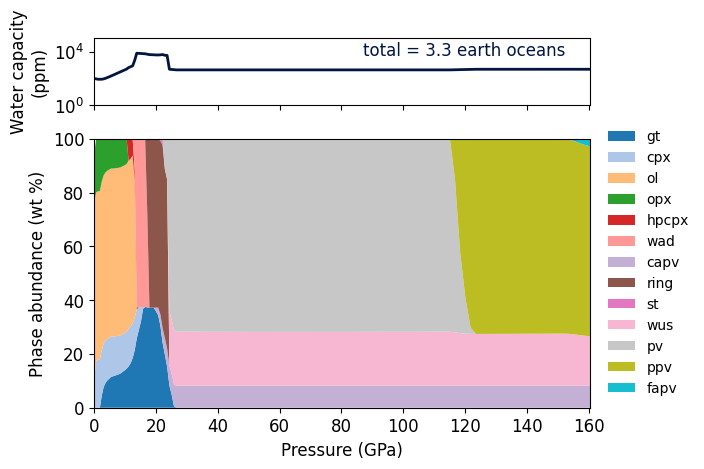
\includegraphics[width=\textwidth]{1M_80Ceff_2MASS19472449+4905040_1600K_modes_c_h2o}
        %  \caption{}
         \label{fig:mgsi_hypatia10}
     \end{subfigure}
    %  \hfill
     \begin{subfigure}[b]{0.6\textwidth}
         \centering
         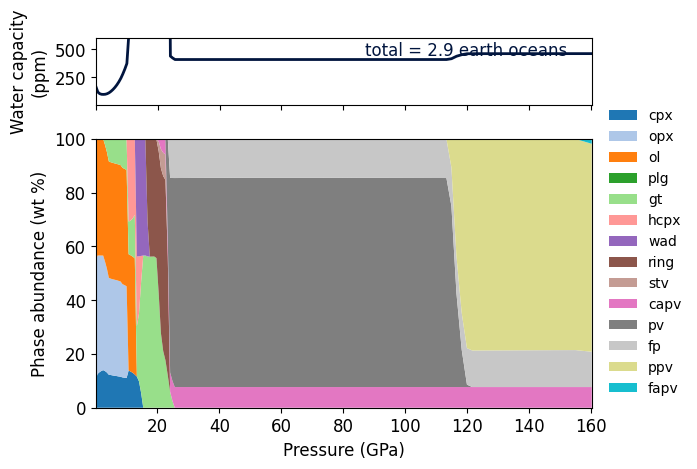
\includegraphics[width=\textwidth]{1M_80Ceff_2MASS19375133+4945541_1600K_modes_c_h2o}
        %  \caption{}
         \label{fig:mgsi_hypatia50}
     \end{subfigure}
    %  \hfill
     \begin{subfigure}[b]{0.6\textwidth}
         \centering
         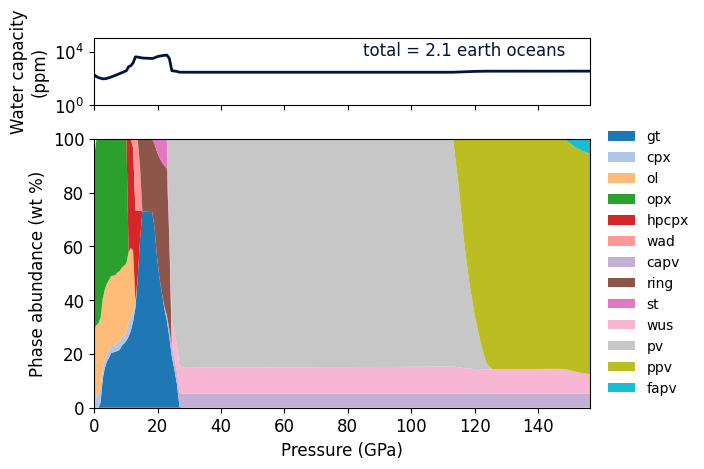
\includegraphics[width=\textwidth]{1M_80Ceff_HIP29295_1600K_modes_c_h2o}
        %  \caption{}
         \label{fig:mgsi_hypatia10}
     \end{subfigure}
        \caption{Samples of mineral phase modalities and water saturation profiles, from \textit{(top)} the 90th percentile, \textit{(centre)} 50th percentile, and \textit{(bottom)} 10th percentile of Mg/Si ratios across the Hypatia catalogue. Shown here are compositions for $T_p = 1600$~K and 1 M_$\oplus$. Increasing the planet mass would extend the lower mantle mineralogies shown to deeper pressures; potential temperatures do not have a large effect on the equilibrium mineralogy. \todo{[or, should hold constant wt\% oxides and just vary Mg/Si? should show some more extreme ``exotic" compositions?]}}
        \label{fig:mgsi_hypatia}
\end{figure}


\subsection{Water storage capacity as a function of planet mass}

\todo{explain mass effect, explain why mass doesn't scale 1:1}

\todo{Figure \ref{fig:violin_masses}}

\todo{Figure \ref{fig:mass_um}}

\todo{Figure \ref{fig:h2o_mgsi_scatter}}

\begin{figure}
\centering
\begin{subfigure}[b]{.5\textwidth}
  \centering
  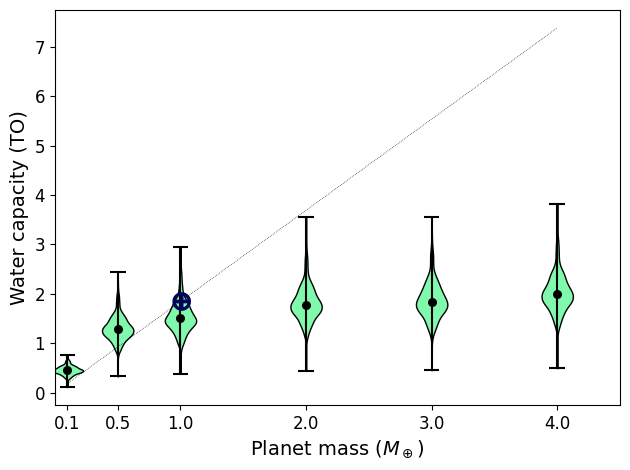
\includegraphics[width=\linewidth]{viol-Mp_w_um.png}
  \caption{}
  \label{fig:violin_um}
\end{subfigure}
\hfill
\begin{subfigure}[b]{.5\textwidth}
  \centering
  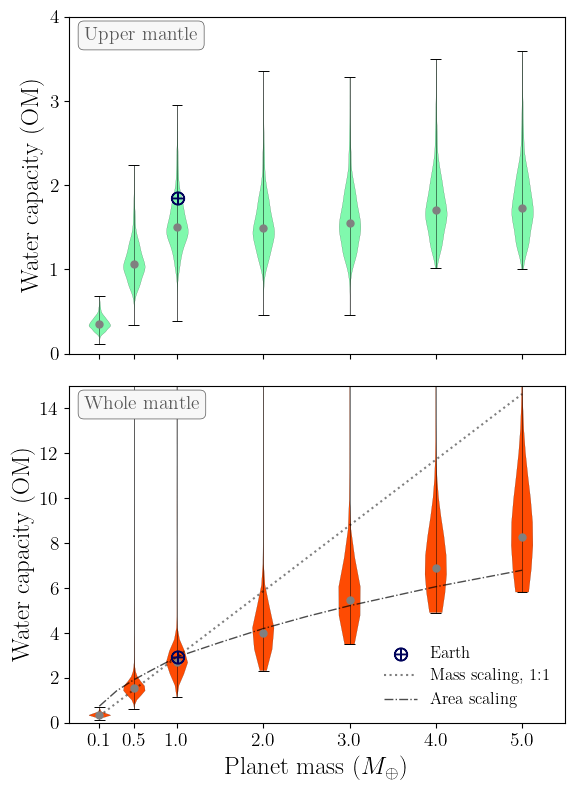
\includegraphics[width=\linewidth]{viol-Mp_w_tot.png}
  \caption{}
  \label{fig:violin_total}
\end{subfigure}
\caption{Distributions across the Hypatia catalogue of upper mantle \textit{(left)} and total mantle \textit{(right)} water storage capacities, as a function of planet mass.}
\label{fig:violin_masses}
\end{figure}


\begin{figure}
    \centering
    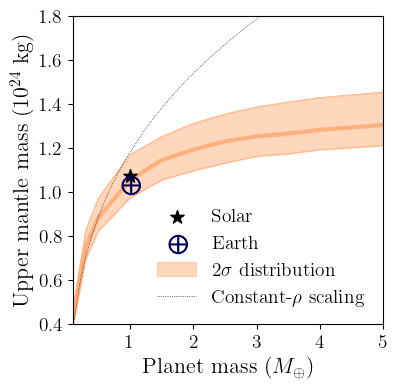
\includegraphics{pops_dist_M_p_mass_um.png}
    \caption{Scaling of the upper mantle mass with the total planet mass. The black line represents a naive scaling assuming a constant mantle density of 4500 kg $m^-3$ and an Earth-like bulk density of 5510 kg $m^-3$.}
    \label{fig:mass_um}
\end{figure}

\begin{figure}
    \centering
    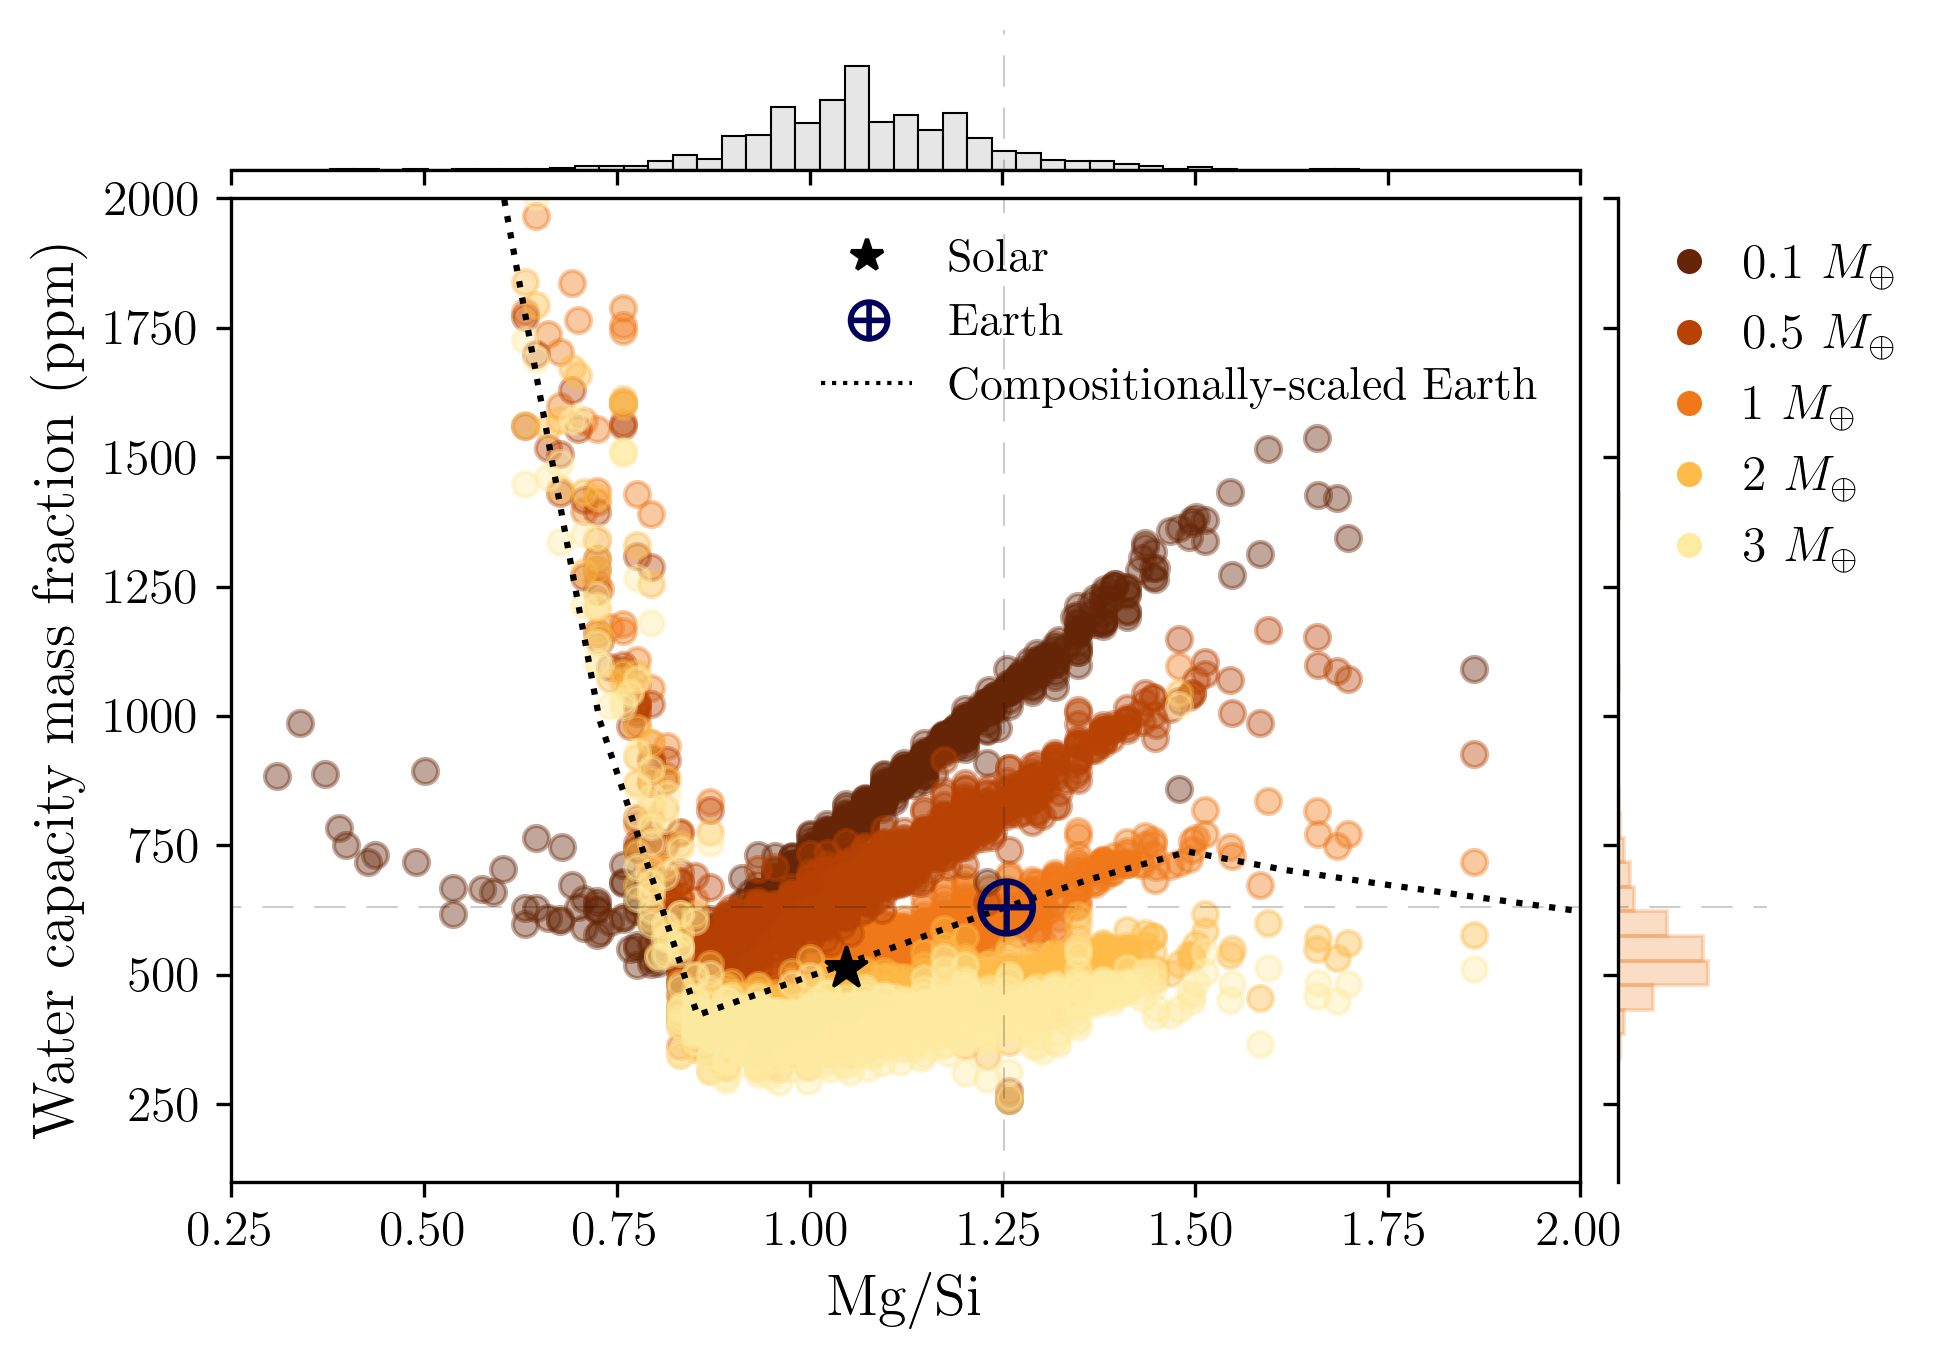
\includegraphics{mgsi_c_h2o_mantle_scatter_all.png}
    \caption{Whole-mantle water storage capacities of each run in terms of the bulk Mg/Si ratio. Colours represent the planet mass.}
    \label{fig:h2o_mgsi_scatter}
\end{figure}

\subsection{Effects of potential temperature and iron fractionation}

\todo{Figure \ref{fig:sat_diff_T}}

\begin{figure}
    \centering
    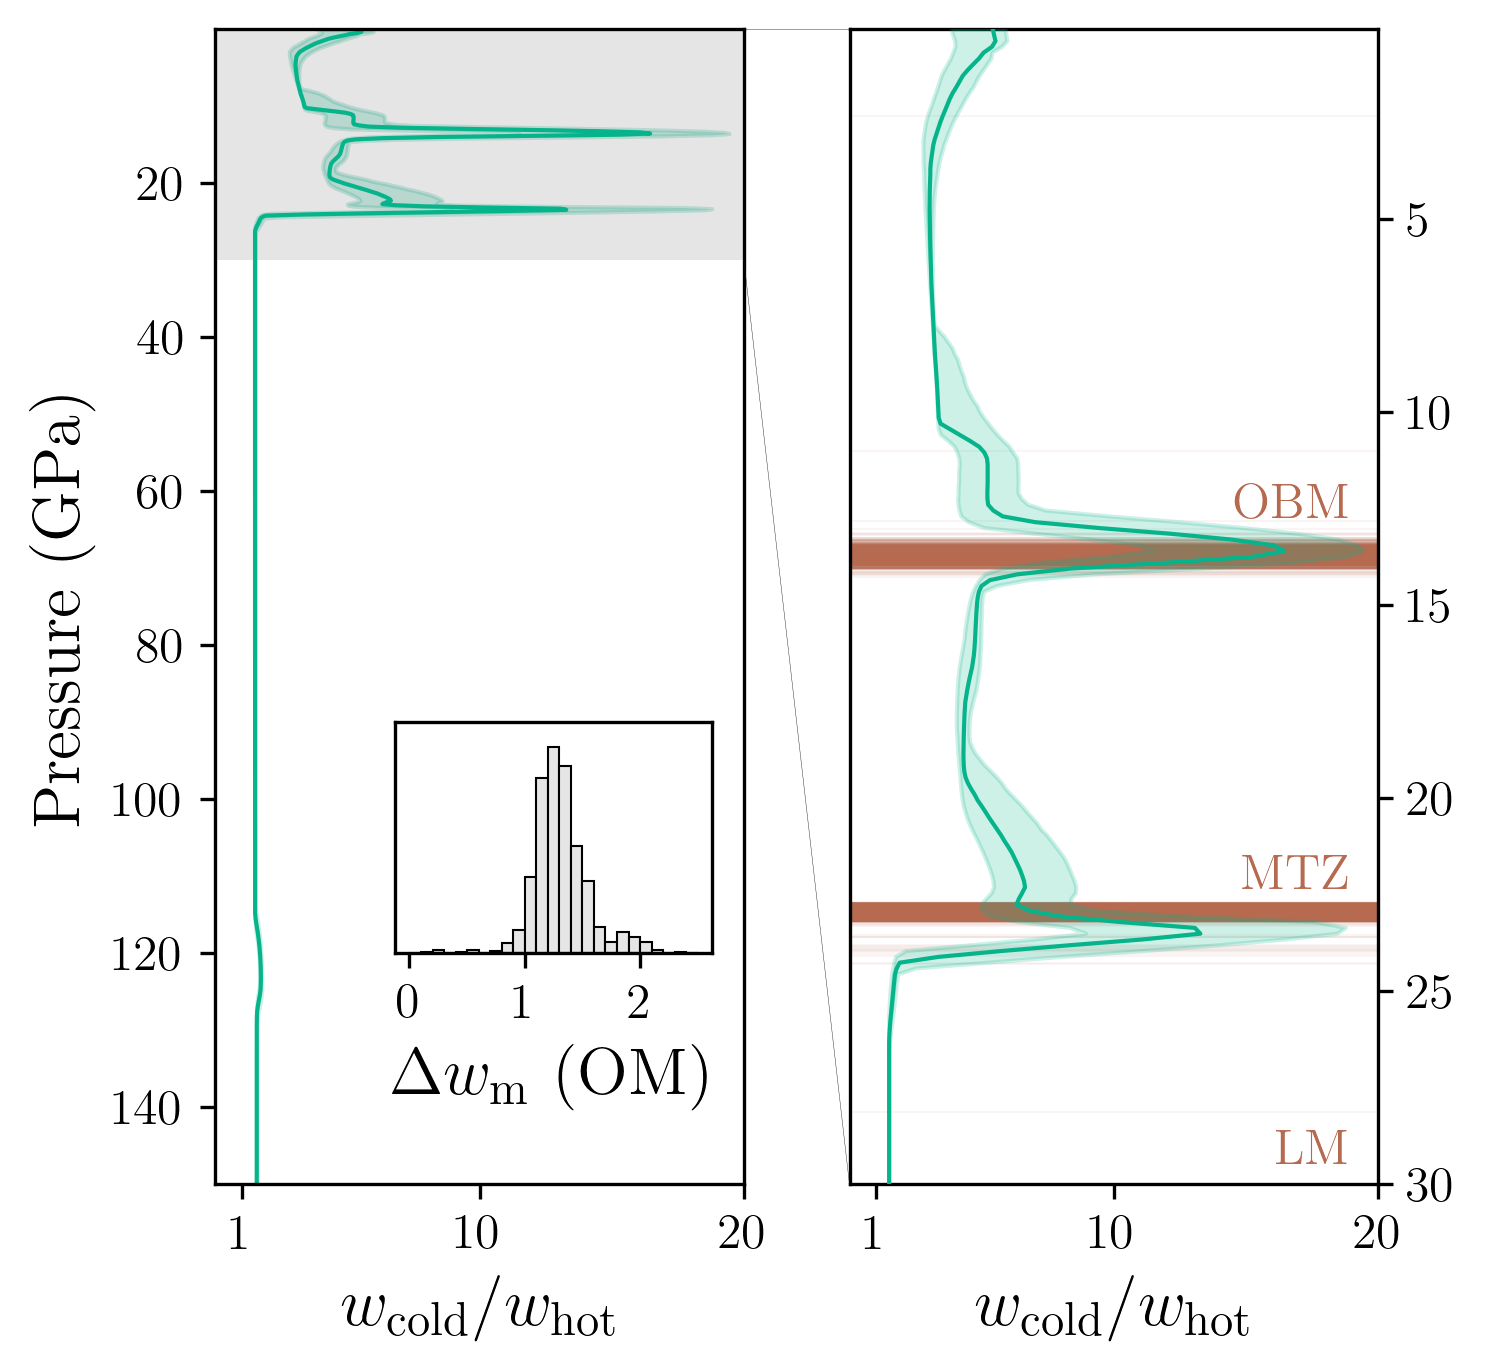
\includegraphics[width=1\textwidth]{sat_T_diff.png}
    \caption{Difference in absolute mantle water capacity profiles between potential temperatures of 1600~K and 1900~K. Shown for a 1-$M_\oplus$ planet, with swaths spanning the 1-$\sigma$ distribution over Hypatia catalog compositions. Increasing the planet mass would roughly extend these lines vertically. \todo{there's a bug in this figure and values shown currently are too low...}}
    \label{fig:sat_diff_T}
\end{figure}

\subsection{Sensitivity to water capacity parameterisations}

\todo{especially garnet, Ca-pv, SiO2 polymorphs}

%Nearly simultaneously with \citet{dong_constraining_2021}, \citet{shah_internal_2021} also fit a water saturation model to experimental data on olivine, wadsleyite, and ringwoodite. The key difference between these two parameterisations is that \citet{shah_internal_2021} find an iron content-dependence of the olivine water capacity, whereas the former do not.


\section{Discussion}


% \subsection{High-pressure phases in the most massive rocky planets, and the likelihood of other exotic minerals}

% Whereas Earth's core-mantle boundary sits at around 136 GPa, pressures in the lower mantles of 5-$M_\Earth$ planets could reach \todo{XX} GPa and \todo{YY} GPa for core mass fractions of 0.33 and 0.1 respectively. Calculating mineral phase assemblages, and associated water capacities, therefore requires extrapolating thermodynamic data beyond Earth-like conditions. This represents a caveat to our study and others interested in rocky planets' compositional diversity. More recently, however, \textit{ab initio} calculations have been used to predict phase transitions of magnesium silicates beyond that of perovskite to postperovskite \citep{umemoto_two-stage_2011, umemoto_phase_2017, van_den_berg_mass-dependent_2019}. \todo{[usefully reviewed in \citet{boujibar_super-earth_2020}]} Although these predictions do not yet account for species other than Mg-endmembers, they will provide a useful benchmark to the extrapolations performed here.

% \todo{need to fix this new bug in model for high masses and set of Tp, and compare to the MgSiO3 phase diagrams in e.g. van den Berg 2019 figure 2}

% The other extrapolation we are performing is in the water capacities of these high-pressure phases, which becomes quite a critical source of uncertainty considering that they will make up more and more of the mantle's total volume for increasing planet mass....

% Finally, it is worth discussing the possibility of wholly alien mineral assemblages. Of course, our modelling is limited to a prescribed set of phases. Nevertheless, the same principles of thermodynamics should apply to every planet no matter what it formed from. That is, even if phase diagrams must be extrapolated, cannot be interpolated to non-native results. For example, \citet{dorn_new_2019} posited that planetary building blocks solidifying above 1200 K could produce mantles much richer in Ca- and Al- bearing minerals, compared to Si-, Mg-dominant Earth. Yet they are able to predict stable assemblages using familiar minerals, so long as the sum of CaO and Al$_2$O$_3$ is less than 80 wt\%. These ultra-refractory planets made of garnet, calcium-ferrite, and calcium-perovskite probably form one end-group of compositional exoticism; the others being very Si-rich planets saturated in quartz, and very Mg-rich planets dominated by magnesiow\"ustite \citep{putirka_composition_2019, putirka_compositional_2021}. 

\subsection{High water capacities of SiO$_2$-rich planets?}


\subsection{Hydrous minerals stable at deep mantle pressures?}

This work has considered water contents from only nominally-anhydrous minerals; that is, water stored as hydrogen in crystal defects, where the maximum solubility is at most $\sim$1 wt\%. However, bona fide hydrous minerals can store over 10 wt\% water as double hydroxide groups, (OH)$_2$, or as OOH groups. These hydrous mineral phases, such as brucite Mg(OH)$_2$, tend to be stable at low pressures found only the very top of the mantle, or at relatively low temperatures found only in subducting slabs \citep[e.g.,][]{hermann_high-pressure_2016}, which are not crossed by our typical geotherms. Hydrous phases stable at crust temperatures will not contribute significantly to the total water budget if the crust makes up \todo{very small total fraction of planet mass... should quantify this assuming 10 wt\% hydration or something}

Some work suggests that there are indeed some hydrous phases stable in the deep mantle... 





% \subsection{Effects of light elements in the core}

% This work has only considered pure iron cores. The presence of light elements in the core---inferred for Mars, and possibly Venus as well as Earth \citep{stahler_seismic_2021, shah_possible_2021}---reduce its density, meaning that the core would occupy a larger volume of the planet for the same bulk planet density, and the \todo{mantle would extend to lower pressures?}. Equilibrium chemistry predicts several weight percent hydrogen sequestering in the core during planetary differentiation \citep{schlichting_chemical_2021}. Further to the interior structure implications, hydrogen in the core would be a ``sink" for primordial water. Nevertheless, this core sink would probably be too inaccessible to participate directly in a planet's deep water cycle over the course of its evolution.

\subsection{Dynamic water}

Because the diversity of rocky exoplanets' water capacities has not been fully explored, many previous studies of their water cycling have taken a high mantle water capacity for granted \citep{cowan_water_2014, schaefer_persistence_2015, moore_keeping_2020}. We have revisited this storage limit, finding that Earth-mass planets may only store at most a few oceans' worth of water in their mantles. Smaller mantle water capacities, more readily reached, would imply more water in the surface and atmosphere reservoirs once the mantle crystallises.

To this end, we have not explicitly considered the dynamics of water: where do we expect it to end up, upon magma ocean crystallisation, or after billions of years of mantle convection? As we have repeated, it is quite possible that magma oceans retain water at their saturation capacity \citep{dorn_hidden_2021}. Hence, as these magma oceans cool, the excess water at each layer (above saturation) will move \todo{either up or down, depending on --- the relative saturation capacity between layers? look at Tikoo paper}



\section{Conclusion}


\bibliographystyle{aasjournal}
\bibliography{references.bib}
\end{document}
